% 9 variables in here:
% h_1 = 10.0, h_2 = 10.0, h_3 = 10.0, ux_1 = 0.0, ux_2 = 3.0, ux_3 = 0.0, uy_1 = 0.0, uy_2 = 3.0, uy_3 = 0.0
\begin{figure}[ht]
\centering
  % \subfigure[] {
  %   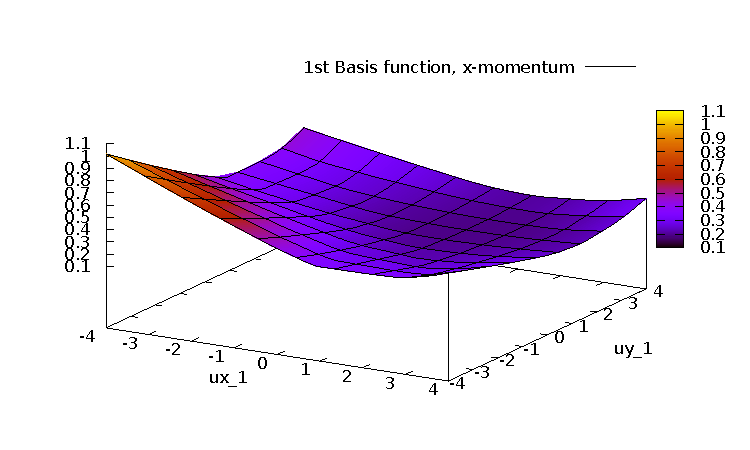
\includegraphics[scale=\zoomfactor]{{{ord1_varying_ux1_uy1_differing_ux2_uy2_3_3/10.0_10.0_10.0_x_3.0_0.0_y_3.0_0.0f0}}}
  % }
  \subfigure[] {
    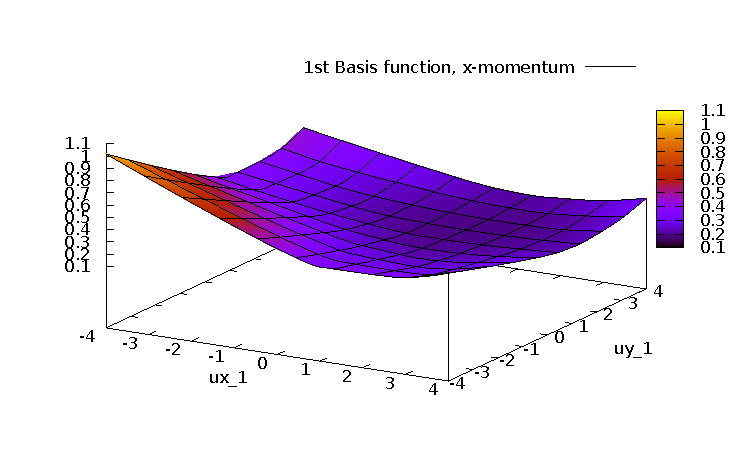
\includegraphics[scale=\zoomfactor]{{{ord1_varying_ux1_uy1_differing_ux2_uy2_3_3/10.0_10.0_10.0_x_3.0_0.0_y_3.0_0.0f00}}}
  }
  \subfigure[] {
    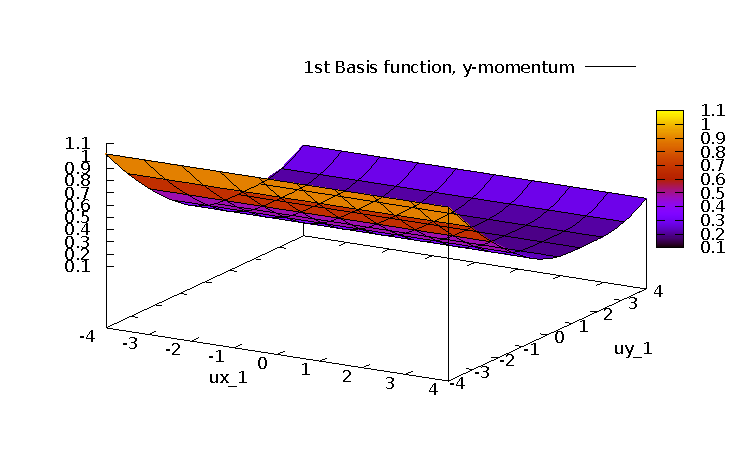
\includegraphics[scale=\zoomfactor]{{{ord1_varying_ux1_uy1_differing_ux2_uy2_3_3/10.0_10.0_10.0_x_3.0_0.0_y_3.0_0.0f01}}}
  }
  \subfigure[] {
    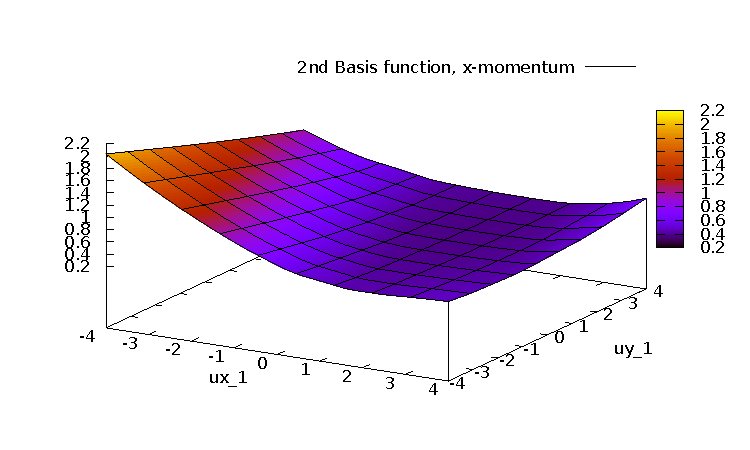
\includegraphics[scale=\zoomfactor]{{{ord1_varying_ux1_uy1_differing_ux2_uy2_3_3/10.0_10.0_10.0_x_3.0_0.0_y_3.0_0.0f02}}}
  }
  \subfigure[] {
    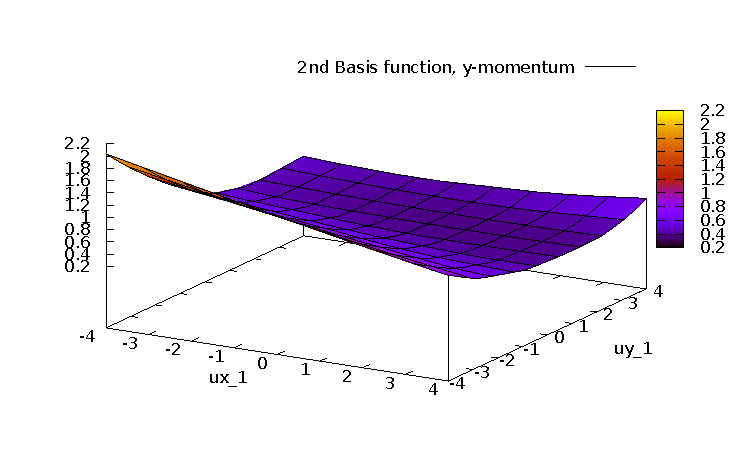
\includegraphics[scale=\zoomfactor]{{{ord1_varying_ux1_uy1_differing_ux2_uy2_3_3/10.0_10.0_10.0_x_3.0_0.0_y_3.0_0.0f03}}}
  }
  \subfigure[] {
    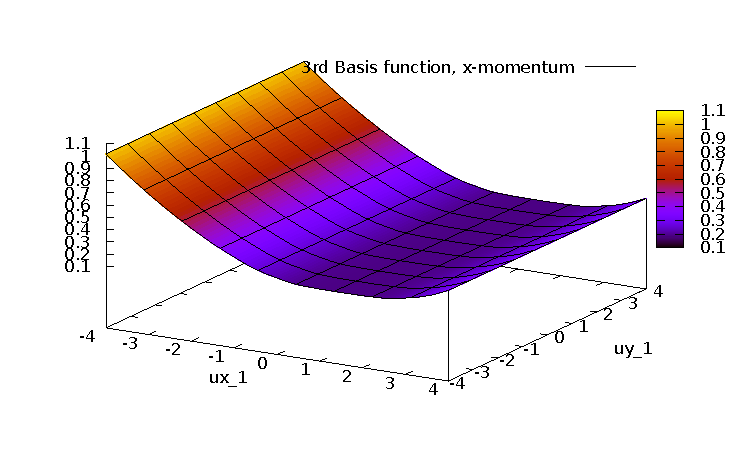
\includegraphics[scale=\zoomfactor]{{{ord1_varying_ux1_uy1_differing_ux2_uy2_3_3/10.0_10.0_10.0_x_3.0_0.0_y_3.0_0.0f04}}}
  }
  \subfigure[] {
    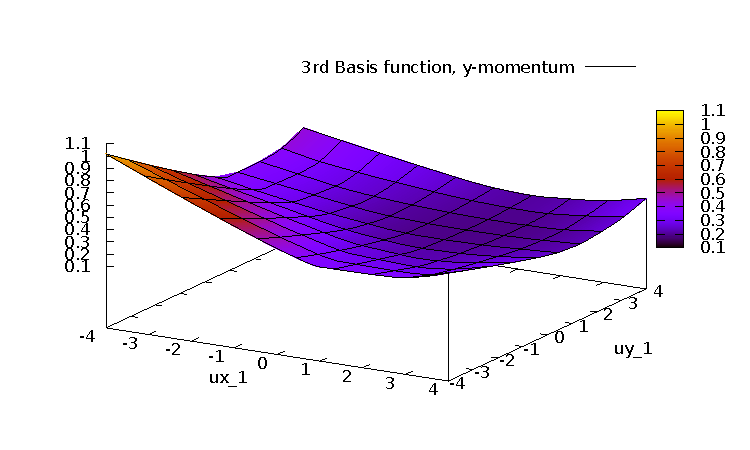
\includegraphics[scale=\zoomfactor]{{{ord1_varying_ux1_uy1_differing_ux2_uy2_3_3/10.0_10.0_10.0_x_3.0_0.0_y_3.0_0.0f05}}}
  }
  % \subfigure[] {
  %   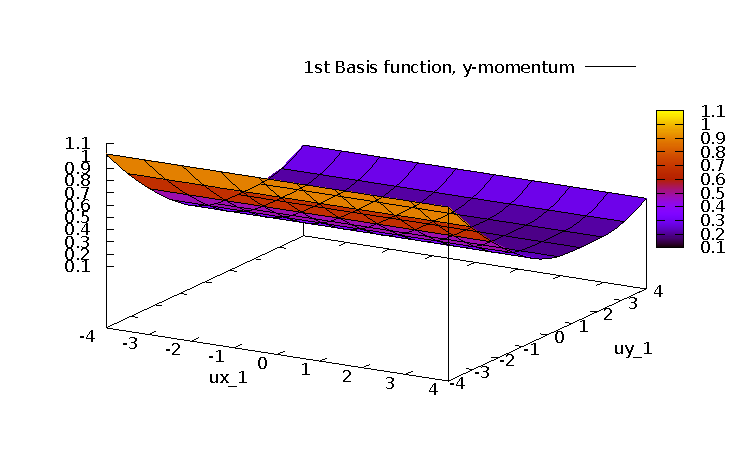
\includegraphics[scale=\zoomfactor]{{{ord1_varying_ux1_uy1_differing_ux2_uy2_3_3/10.0_10.0_10.0_x_3.0_0.0_y_3.0_0.0f1}}}
  % }
  % \subfigure[] {
  %   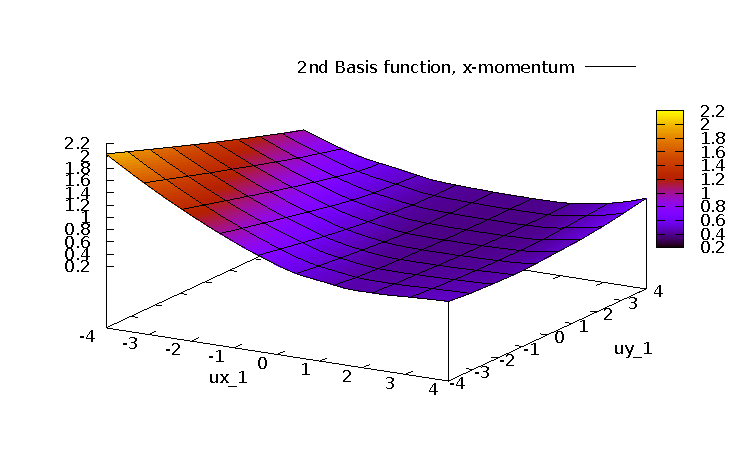
\includegraphics[scale=\zoomfactor]{{{ord1_varying_ux1_uy1_differing_ux2_uy2_3_3/10.0_10.0_10.0_x_3.0_0.0_y_3.0_0.0f2}}}
  % }
  % \subfigure[] {
  %   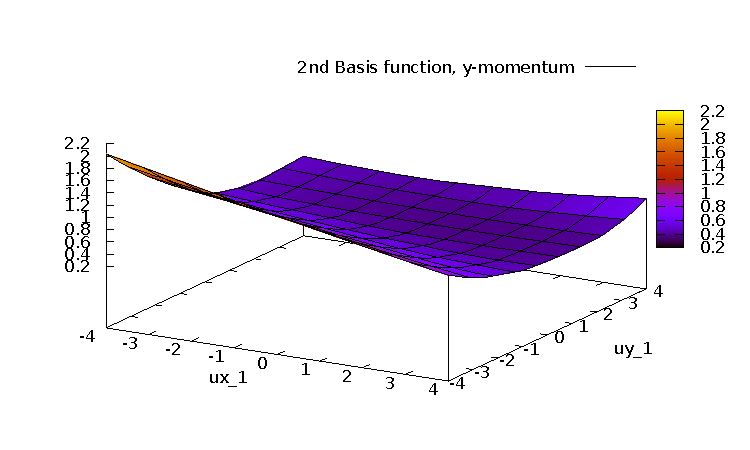
\includegraphics[scale=\zoomfactor]{{{ord1_varying_ux1_uy1_differing_ux2_uy2_3_3/10.0_10.0_10.0_x_3.0_0.0_y_3.0_0.0f3}}}
  % }
  % \subfigure[] {
  %   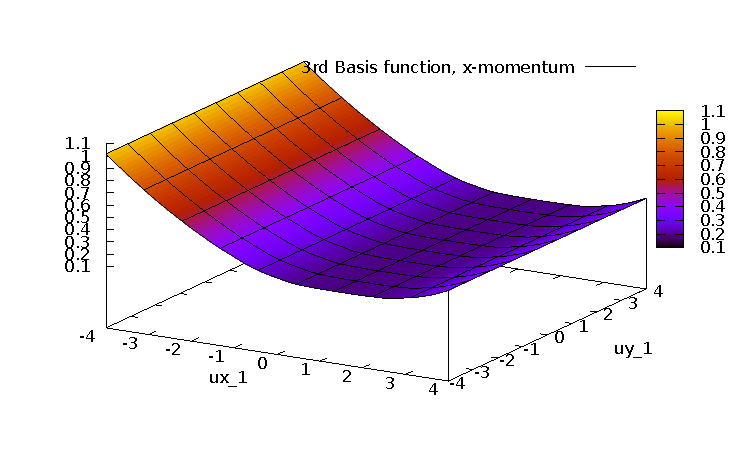
\includegraphics[scale=\zoomfactor]{{{ord1_varying_ux1_uy1_differing_ux2_uy2_3_3/10.0_10.0_10.0_x_3.0_0.0_y_3.0_0.0f4}}}
  % }
  % \subfigure[] {
  %   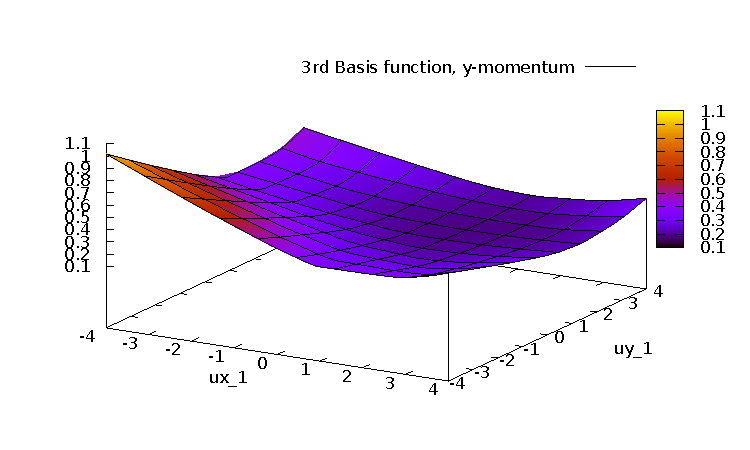
\includegraphics[scale=\zoomfactor]{{{ord1_varying_ux1_uy1_differing_ux2_uy2_3_3/10.0_10.0_10.0_x_3.0_0.0_y_3.0_0.0f5}}}
  % }
\caption{All heights are 10, $u_{x,2}=u_{y,2}=3$, $u_{x,3}=u_{y,3}=0$. We omitted the plot for $y$-momentum with the third basis function since it looks like the one for the $x$-momentum of the first basis function. Moreover, we omitted the $x$-plot for the third basis function -- it looks like the $y$-plot for the first basis function mirrored at the plane $u_{x,1}=u_{x,2}$. The $y$-plot for the second basis function looks like the $x$-plot for the second basis function mirrored at the plane $u_{x,1}=u_{x,2}$.}
\label{fig:ord1_varying_ux1_uy1_differing_ux2_uy2_3_3}
\end{figure}

%%% Local Variables:
%%% TeX-master: "../results.tex"
%%% End:
